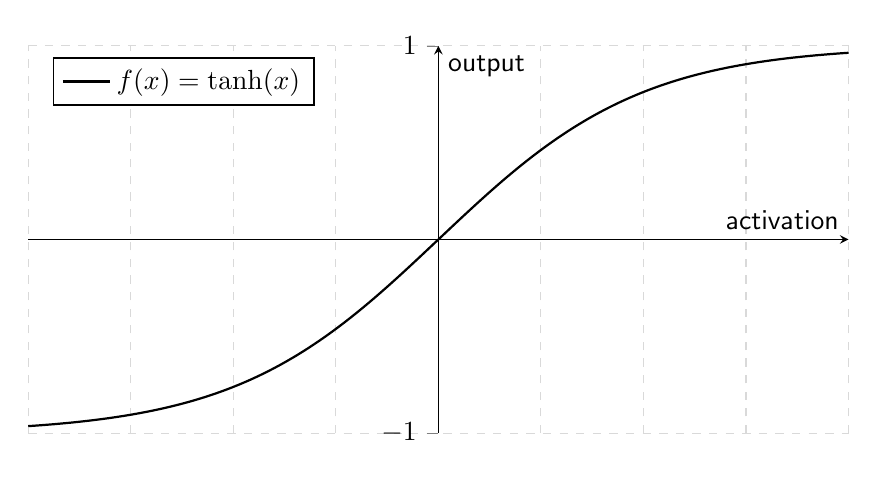
\begin{tikzpicture}[font=\sffamily]
    \begin{axis}[
    	legend pos=north west,
        axis x line=middle,
        axis y line=middle,
        grid = major,
        width=12cm,
        height=6.5cm,
        grid style={dashed, gray!30},
        xmin=-2,xmax= 2,ymin= -1,ymax= 1,
        xlabel=activation,ylabel=output,
        tick align=outside,
        ytick={-1,1},
        xmajorticks=false,
        enlargelimits=false]
      \addplot[domain=-2:2,black,thick,samples=500] {tanh(x)}; 
      \addlegendentry{$f(x)=\tanh(x)$}
    \end{axis} 
\end{tikzpicture}